\documentclass[beamer]{standalone}
\usepackage{circuitikz}
\begin{document}

\title[Electronics 1]{Transistors and AC amplifiers}

\begin{frame} 
  \titlepage
\end{frame}

\section{Bipolar junction Transistor (BJT)}
\begin{frame}
\frametitle{Transistors}
\begin{itemize}
	\item invented in 1947
	\item replaced vacuum tube 
	\item \alert{amplify current}
	\item lower power consumption
	\item cheap for mass production
	\item robust to vibration
	\item long working time (decades) when properly used
	\item building block of modern electronics
\end{itemize}
Some areas where vacuum tube are still good
\begin{itemize}
	\item ultra high voltage applications (more than 1000 V)
	\item radiation prone locations
\end{itemize}
\end{frame}
	
\begin{frame}
\frametitle{Bipolar junction Transistor (BJT)}
\begin{columns}[t]
	\begin{column}{.5\textwidth}
		NPN-transistor
		\begin{columns}[t]
			\begin{column}{.40\textwidth}
				\begin{figure}
					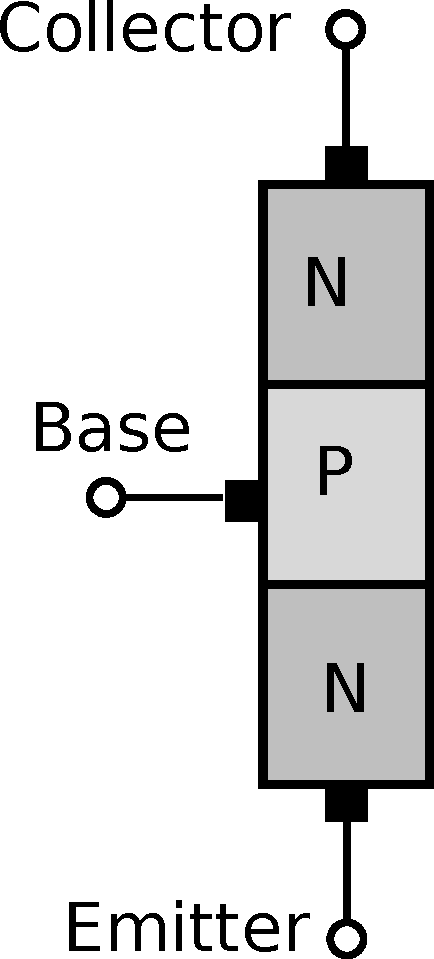
\includegraphics[width=0.80\textwidth]{./pics/npn_transistor.pdf}
				\end{figure}
			\end{column}
			\begin{column}{.60\textwidth}
				\begin{figure}
					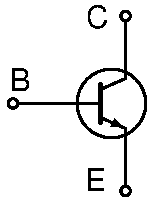
\includegraphics[width=0.80\textwidth]{./schematics/npn_transistor.pdf}
				\end{figure}
				\begin{figure}
					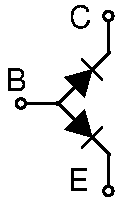
\includegraphics[width=0.30\textwidth]{./schematics/npn_diodes.pdf}
				\end{figure}
			\end{column}
		\end{columns}

	\end{column}
	\begin{column}{.5\textwidth}
		PNP-transistor
		\begin{columns}[t]
			\begin{column}{.40\textwidth}
				\begin{figure}
					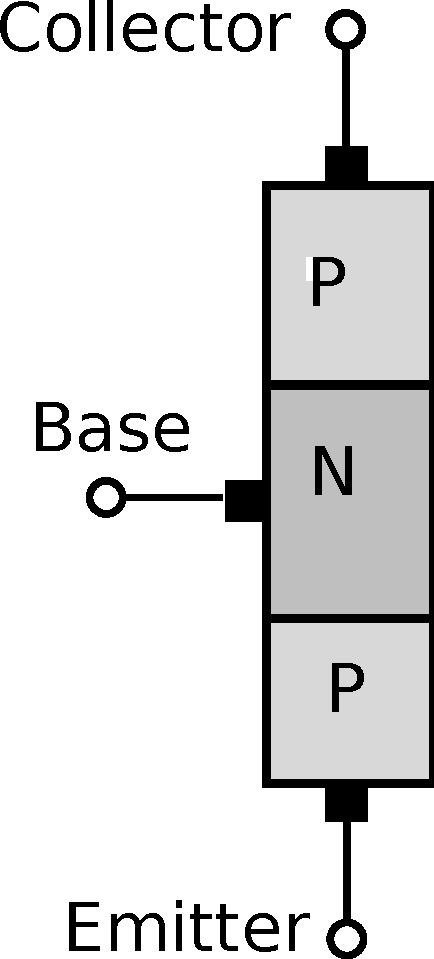
\includegraphics[width=0.80\textwidth]{./pics/pnp_transistor.pdf}
				\end{figure}
			\end{column}
			\begin{column}{.60\textwidth}
				\begin{figure}
					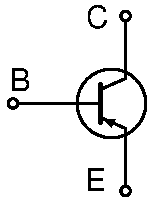
\includegraphics[width=0.80\textwidth]{./schematics/pnp_transistor.pdf}
				\end{figure}
				\begin{figure}
					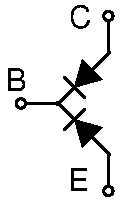
\includegraphics[width=0.30\textwidth]{./schematics/pnp_diodes.pdf}
				\end{figure}
			\end{column}
		\end{columns}
	\end{column}
\end{columns}
\end{frame}

\begin{frame}
\frametitle{Notation}
\begin{columns}[t]
	\begin{column}{.65\textwidth}
		\begin{itemize}
			\item Base-emitter current ($I_{be}$)
			\item Collector-emitter current ($I_{ce}$)
			\item Base-emitter voltage difference ($V_{be}=V_b-V_e$)
			\item Collector-emitter voltage difference ($V_{ce}=V_c-V_e$)
		\end{itemize}
	\end{column}
	\begin{column}{.35\textwidth}
		\begin{figure}
			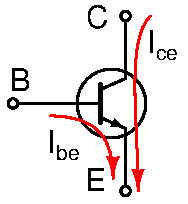
\includegraphics[width=0.80\textwidth]{./schematics/npn_transistor_with_currents.pdf}
		\end{figure}
	\end{column}
\end{columns}
\end{frame}

\section{Simple rules for transistors circuits} 
\begin{frame}
\frametitle{Simple NPN-transistor rules}
\begin{columns}[t]
	\begin{column}{.75\textwidth}
		To support shown currents direction
		\begin{itemize}
			\item<2-> \alert{$V_{ce} > 0$}
			\item<3-> \alert{$V_{be} > 0$}
				\begin{itemize}
					\item since, it is forward biased diode $V_{be} \approx 0.6$~V
				\end{itemize}
			\item<4-> \alert{$V_{cb} > 0$}
				\begin{itemize}
					\item since, it is reversed biased diode, no current goes from
						collector to base, all collector current is directed to emitter 
					\item if \textcolor{blue}{$V_{cb} < 0$} transistor goes to
						\textcolor{blue}{saturation} and cannot be
						described by the following simple rule.
				\end{itemize}
		\end{itemize}
		\onslide<5->{If above holds true then}
		\begin{itemize}
			\item<6-> \alert{$I_{ce}=\beta I_{be}$} thus a BJT is a current
				amplifier
			\item<7-> {\it the static forward current transfer ratio}\\
				$\beta$ (or sometimes $h_{fe}$)   $\approx 100 \ldots 200$ 
			\item<8-> $I_e = I_{be} + I_{ce} = (\beta+1) I_{be} \approx \beta I_{be}$
		\end{itemize}

	\end{column}
	\begin{column}{.25\textwidth}
		\begin{figure}
			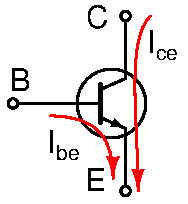
\includegraphics[width=0.80\textwidth]{./schematics/npn_transistor_with_currents.pdf}
		\end{figure}
		\begin{figure}
			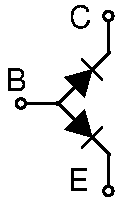
\includegraphics[width=0.40\textwidth]{./schematics/npn_diodes.pdf}
		\end{figure}

	\end{column}
\end{columns}
\end{frame}
	
\begin{frame}
\frametitle{Simple PNP-transistor rules}
\begin{columns}[t]
	\begin{column}{.65\textwidth}
		Apply the same rules as before for NPN BJT but multiply currents and voltages by
		-1.

		Hints 
		\begin{itemize}
			\item 
				the arrow indicates the direction in which current is supposed to
				flow.
			\item 
				the arrow always connects the base and emitter.
		\end{itemize}
	\end{column}
	\begin{column}{.25\textwidth}
		\begin{figure}
			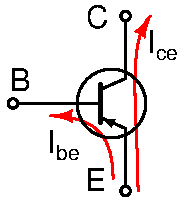
\includegraphics[width=0.80\textwidth]{./schematics/pnp_transistor_with_currents.pdf}
		\end{figure}
		\begin{figure}
			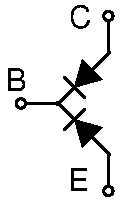
\includegraphics[width=0.40\textwidth]{./schematics/pnp_diodes.pdf}
		\end{figure}
	\end{column}
\end{columns}
\end{frame}

\begin{frame}
\frametitle{Design considerations for $\beta$}
Remember \alert{$\beta$ is not a constant!}

It depends on many parameters
\begin{itemize}
	\item temperature
	\item collector current
	\item varies from device to device even in the same batch
\end{itemize}

Good design should not depend on $\beta$ value.
\end{frame}

\section{Constant current source}	
\begin{frame}
\frametitle{Constant current source}
	\begin{columns}[c]
		\begin{column}{.35\textwidth}
			\begin{figure}
				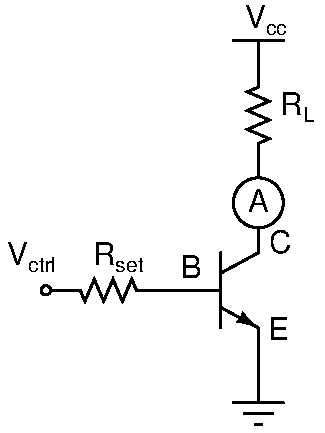
\includegraphics[height=0.60\textheight]{./schematics/npn_constant_current_source.pdf}
			\end{figure}

		\end{column}
		\begin{column}{.65\textwidth}
			Current through the load resistor does not depend on the load
			resistance.

			\begin{equation*}
				I_L= I_{ce} = \beta I_{be} = \beta \frac{V_{ctrl}-.6V}{R_{set}} 
			\end{equation*}

			\onslide<2->{
			This is actually a sample of \alert{bad design} since the current through the
			load \alert{ depends on $\beta$}.
			}

			\onslide<3->{
			\[
			V_c = V_{cc} - R_L I_L 
			\]
			}

			\onslide<4->{
			Remember that $V_c$ must be $> V_b$
			thus current  cannot be bigger than the saturation current
			\[
			I_{sat} = max(I_L) \le \frac{V_{cc} - V_{b}}{R_L} \approx \frac{V_{cc}}{R_L}
			\]
			}

		\end{column}
	\end{columns}
\end{frame}
	
\begin{frame}
\frametitle{Constant current source (continued)}
	\begin{columns}[c]
		\begin{column}{.25\textwidth}
			\begin{figure}
				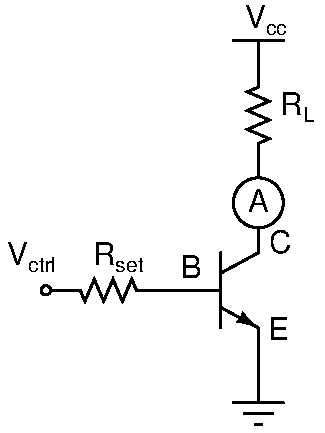
\includegraphics[height=0.30\textheight]{./schematics/npn_constant_current_source.pdf}
			\end{figure}
		\end{column}
		\begin{column}{.6\textwidth}
			From $V_{cc}$ point of view,
			left schematic is equivalent to the right one.
			\[
			R_{trans} = \frac{ V_{ce}} {I_L}
			= \frac{V_{cc} - I_L R_L}{I_L}
			\]
			\begin{block}{Transistor}
				{\bf Tran}(sform)-(re){\bf sistor}
			\end{block}
		\end{column}
		\begin{column}{.25\textwidth}
			\begin{figure}
				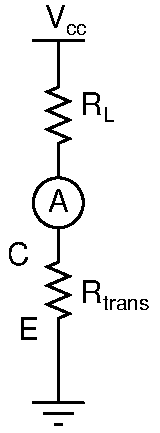
\includegraphics[height=0.30\textheight]{./schematics/npn_constant_current_source_equivalent.pdf}
			\end{figure}
		\end{column}
	\end{columns}
\end{frame}

\begin{frame}
\frametitle{Constant current source. Power dissipation.}
			Transistor power dissipation
	\begin{columns}[c]
		\begin{column}{.25\textwidth}
			\begin{figure}
				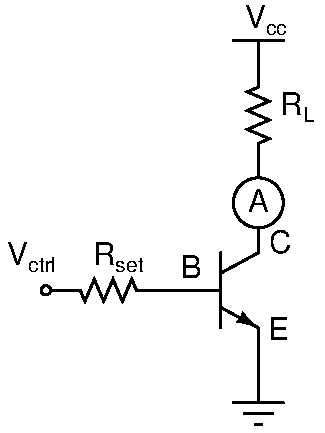
\includegraphics[height=0.30\textheight]{./schematics/npn_constant_current_source.pdf}
			\end{figure}
		\end{column}
		\begin{column}{.6\textwidth}

			\[P_{trans} = P_{be} + P_{ce} = V_{be} I_{be} + V_{ce} I_{ce} \]

			Since \\
			$V_{be} \le V_{ce}$ , $I_{be} = I_{ce}/\beta \ll I_{ce}$, and
			$I_{ce}=I_L$

			\[P_{trans} \approx  V_{ce} I_{ce} = R_{trans} I^2_{L}\]

			\onslide<2->{
			Maximum power dissipation in transistor 
			}
			\onslide<3->{
			is when $R_{trans}=R_L$
			}
			\onslide<4->{
			\[
			max(P_{trans}) = \frac{V_{cc}^2 }{4 R_L}, ~\mathrm{when}~
			I_L=\frac{V_{cc}}{2 R_L} 
			\]
			}

		\end{column}
		\begin{column}{.25\textwidth}
			\begin{figure}
				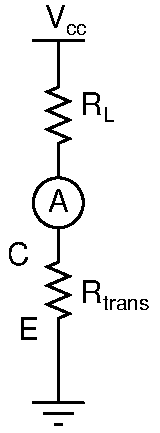
\includegraphics[height=0.30\textheight]{./schematics/npn_constant_current_source_equivalent.pdf}
			\end{figure}
		\end{column}
	\end{columns}
\end{frame}

\section{Voltage controlled switch}	
\begin{frame}
\frametitle{Voltage controlled switch}
	When properly designed outcome does not depend on reasonable variations
	of $\beta$
	\begin{columns}[c]
		\begin{column}{.3\textwidth}
			\begin{figure}
				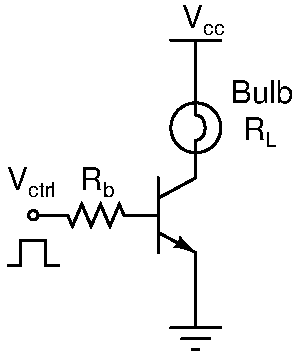
\includegraphics[height=0.40\textheight]{./schematics/npn_switch.pdf}
			\end{figure}

		\end{column}
		\begin{column}{.70\textwidth}
			Recall that typically $\beta = 100 \ldots 200$

			We will assume the worst case scenario \alert{$\beta=10$}

			Notice that $R_L$ limits collector current
			\[ I_L = \frac{V_{cc}}{R_L} \]
			\begin{equation*}
				I_{be} = \frac{V_{ctrl}-.6V}{R_{b}} =  \frac{I_L}{\beta} 
			\end{equation*}
			\begin{equation*}
				R_b \le \frac{V_{ctrl}-.6V} {V_{cc}} \beta R_L
			\end{equation*}

		\end{column}
	\end{columns}
\end{frame}
	
\section{Emitter follower}	
\begin{frame}
 \frametitle{Emitter follower}
	\begin{columns}[c]
		\begin{column}{.35\textwidth}
			\begin{figure}
				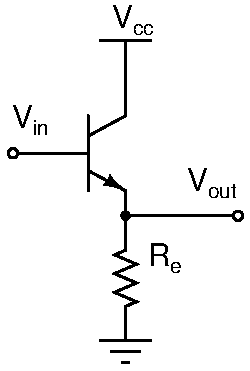
\includegraphics[height=0.60\textheight]{./schematics/npn_emitter_follower.pdf}
			\end{figure}

		\end{column}
		\begin{column}{.65\textwidth}
			\begin{equation*}
				V_{out}=V_{in}-0.6V
			\end{equation*}

			\onslide<2->{ Gain. What gain?}

			\onslide<3->{
			We achieved the input impedance increase.
			\[
			R_{input}=\frac{V_{in}}{I_{be}} \approx R_L (\beta+1)
			\]
			As a result our $V_{in}$ source is not overloaded and our load receive
			all required current (as long as the collector power supply can
			support it).
			}

		\end{column}
	\end{columns}
\end{frame}
	

\frame
{ \frametitle{Summary of simple emitter follower}
\begin{columns}[c]
	\begin{column}{.3\textwidth}
		\begin{figure}
			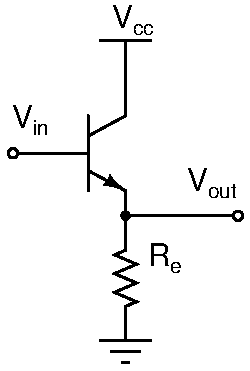
\includegraphics[height=0.60\textheight]{./schematics/npn_emitter_follower}
		\end{figure}
	\end{column}
	\begin{column}<1->{.35\textwidth}
		Advantages
		\begin{itemize}
			\item input impedance increase $Z_{in}=\beta R_e$
			\item power/current gain
			\item output does not depend on $\beta$
			\item simple
		\end{itemize}

	\end{column}
	\begin{column}<2->{.35\textwidth}
		Disadvantages
		\begin{itemize}
			\item input signal must be positive
				\begin{itemize}
					\item even more it should be above 0.6~V
				\end{itemize}
			\item \alert{no voltage gain}
		\end{itemize}
	\end{column}
\end{columns}
	}
	
\frame
{ \frametitle{Real life signal}
	In real life signals usually swing around zero. 

	\vskip .5in
	\pause
	We need to do something with our simple emitter follower.

	\vskip .5in
	\pause 
	Solution 1: Push-Pull follower

	\pause 
	Solution 2: AC-coupled biased-amplifier
	}

\section{NPN and PNP emitter follower}
\frame
{ \frametitle{NPN and PNP emitter follower}
\vskip -.2in
\begin{columns}[c]
	\begin{column}{.30\textwidth}
		NPN emitter follower
	\end{column}
	\begin{column}{.25\textwidth}
		\begin{figure}
			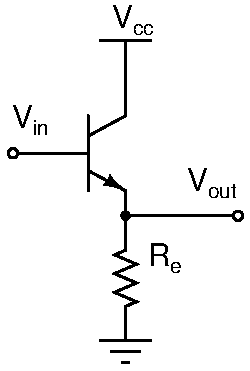
\includegraphics[height=0.30\textheight]{./schematics/npn_emitter_follower}
		\end{figure}
	\end{column}
	\begin{column}<2->{.45\textwidth}
		\begin{figure}
			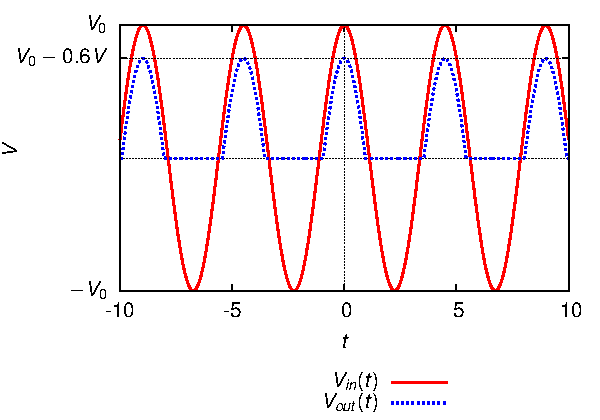
\includegraphics[width=1.00\textwidth,angle=0]{./plots/npn_follower}
		\end{figure}
	\end{column}
\end{columns}
%\vskip -.4in
\begin{columns}[c]
	\begin{column}<3->{.30\textwidth}
		PNP emitter follower
	\end{column}
	\begin{column}<3->{.25\textwidth}
		\begin{figure}
			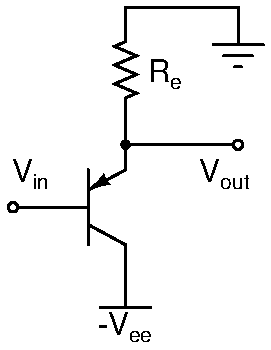
\includegraphics[height=0.30\textheight]{./schematics/pnp_emitter_follower}
		\end{figure}
	\end{column}
	\begin{column}<4->{.45\textwidth}
		\begin{figure}
			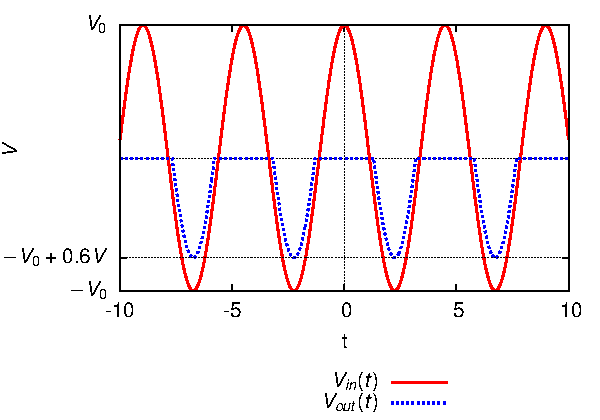
\includegraphics[width=1.00\textwidth,angle=0]{./plots/pnp_follower}
		\end{figure}
	\end{column}
\end{columns}
	}

\section{Push-Pull emitter follower}
\frame
{ \frametitle{Push-Pull emitter follower}
\vskip -.4in
\begin{columns}[c]
	\begin{column}{.30\textwidth}
		\begin{figure}
			\includegraphics<1->[height=0.50\textheight]{./schematics/push_pull_follower}
		\end{figure}
	\end{column}
	\begin{column}<2->{.70\textwidth}
		\begin{figure}
			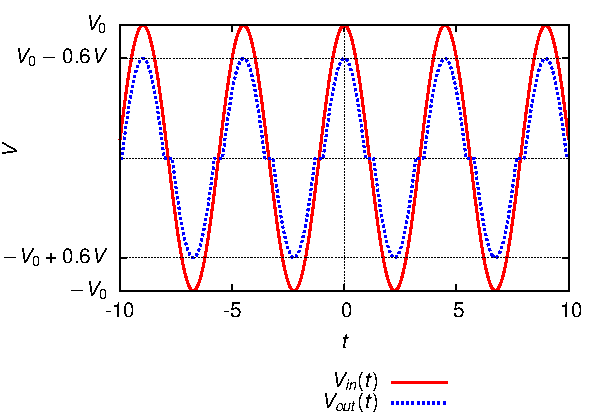
\includegraphics[width=1.00\textwidth,angle=0]{./plots/push_pull_follower}
		\end{figure}
	\end{column}
\end{columns}
	}

\frame
{ \frametitle{Push-Pull follower crossovers}
		\framezoom<2><3>[border](3.9cm, 2.7cm)(1cm, 1cm)
			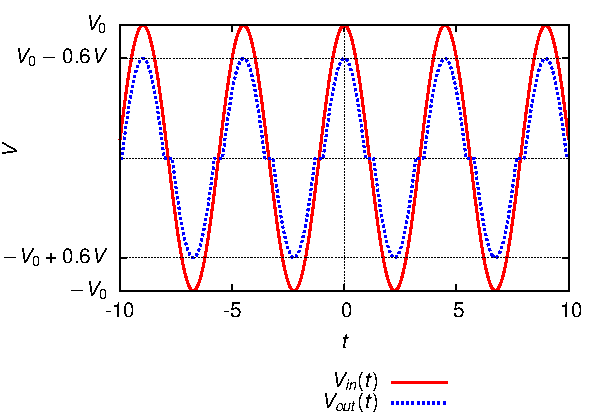
\includegraphics[width=12cm,angle=0]{./plots/push_pull_follower}
	}

\frame
{ \frametitle{Push-Pull emitter follower improved}
\vskip -.4in
\begin{columns}[c]
	\begin{column}{.45\textwidth}
		\begin{figure}
			\includegraphics<1->[height=0.50\textheight]{./schematics/push_pull_follower}
		\end{figure}
	\end{column}
	\begin{column}<2->{.45\textwidth}
		\begin{figure}
			\includegraphics<1->[height=0.50\textheight]{./schematics/push_pull_follower_with_diodes}
		\end{figure}
	\end{column}
\end{columns}
}
	
\section{AC emitter followers}
\frame
{ \frametitle{AC-coupled emitter follower}
\begin{columns}[c]
	\begin{column}{.45\textwidth}
		\begin{figure}
			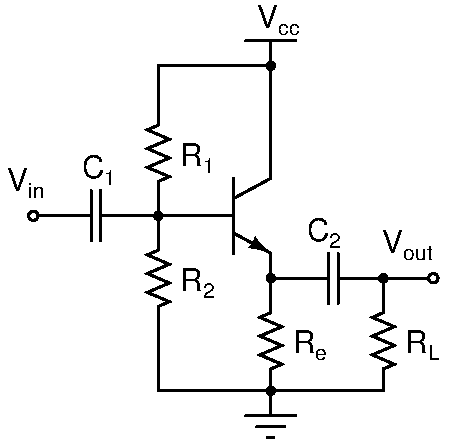
\includegraphics[height=0.50\textheight]{./schematics/npn_ac_emitter_follower}
		\end{figure}
	\end{column}
	\begin{column}<2->{.55\textwidth}
		Design rules
		\begin{itemize}
			\item maximum output swing 
				\begin{itemize}
					\item $V_e=V_{cc} /2 $
				\end{itemize}
			\item disregarding  $V_{be}=0.6$~V
				\begin{itemize}
					\item $V_b \approx V_e=V_{cc}/{2}$
					\item thus $R_1=R_2$
				\end{itemize}
			\item quiescent current
				$I_e=V_e/R_e$
			\item we want $I_{R_1+R_2} \gg I_b$
				\begin{itemize}
					\item factor of 10 for a safe margin
						$I_{R_1+R_2} \ge 10 I_b = 10 I_e / \beta$
					\item thus $R_1=R_2 \le  R_e\beta /10$
				\end{itemize}
		\end{itemize}
	\end{column}
\end{columns}
	
	}

\frame
{ \frametitle{AC-coupled emitter follower: capacitors choice}
\begin{columns}[t]
	\begin{column}{.45\textwidth}
		\vskip -0.4in
		\begin{figure}
			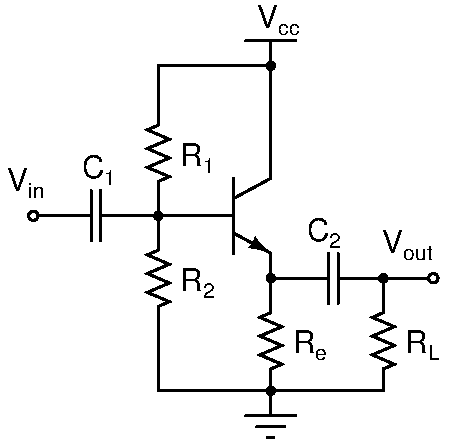
\includegraphics[height=0.40\textheight]{./schematics/npn_ac_emitter_follower}
		\end{figure}
		\vskip -0.3in
		\begin{figure}
			\includegraphics<2->[height=0.20\textheight]{./schematics/ac_coupled_input}
		\end{figure}
		\vskip -0.3in
		\begin{figure}
			\includegraphics<3->[height=0.20\textheight]{./schematics/ac_coupled_output}
		\end{figure}
	\end{column}
	\begin{column}<2->{.55\textwidth}
		From AC point of view
		\begin{itemize}
			\item<2-> Input is RC high-pass
				\begin{itemize}
					\item $C=C_1$
					\item $R=R_1||R_2||\beta R_e$
					\item $f_{3db}=\frac{1}{2 \pi} \frac{1}{C_1 (R_1||R_2||\beta R_e)}$
						\begin{itemize}
							\item with above rules $R \approx R_1/2$
						\end{itemize}
				\end{itemize}
			\item<3-> Output is also RC high-pass
				\begin{itemize}
					\item $C=C_2$
					\item $R=R_L$
					\item $f_{3db}=\frac{1}{2 \pi} \frac{1}{C_2 R_L}$
					\item for unloaded filter $R_L \gg R_e$ 
						\begin{itemize}
							\item factor of 10 for a safe margin
								$R_L = 10 R_e$
						\end{itemize}
				\end{itemize}
		\end{itemize}
	\end{column}
\end{columns}
	
	}
	
\section{Common emitter (inverting) amplifier}
\frame
{ \frametitle{Common emitter (inverting) amplifier}
\begin{columns}[c]
	\begin{column}{.35\textwidth}
		\begin{figure}
			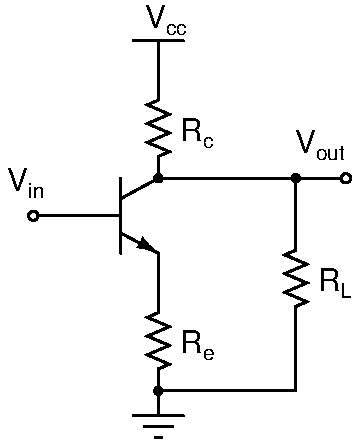
\includegraphics[height=0.50\textheight]{./schematics/npn_common_emitter_amplifier}
		\end{figure}
	\end{column}
	\begin{column}<2->{.65\textwidth}
		\begin{itemize}
			\item $I_c=I_e=(V_{in}-0.6V)/R_e$		
			\item $V_{out}=V_{cc}-R_c I_c$
			\item $V_{out}=V_{cc}-R_c (V_{in}-0.6V)/R_e$
			\item $V_{out}=(V_{cc}+(0.6V) R_c/R_e) -V_{in} R_c/R_e$
			\item gain $G=-R_c/R_e$
			\item attractive to put $R_e=0$
			\begin{itemize}
				\item transistor model fails
				\item transistor emitter resistance $r_e=25mV/I_c$
				\item gain $G=-R_c/r_e$
			\end{itemize}
		\end{itemize}
	\end{column}
\end{columns}
	
	}

\frame
{ \frametitle{Common emitter  amplifier signal output impedance}
\begin{columns}[c]
	\begin{column}{.35\textwidth}
		\begin{figure}
			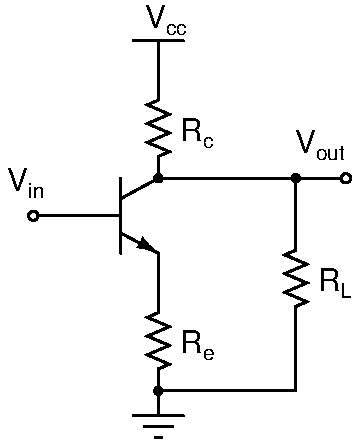
\includegraphics[height=0.50\textheight]{./schematics/npn_common_emitter_amplifier}
		\end{figure}
	\end{column}
	\begin{column}<2->{.65\textwidth}
		\pause
		In the pass band we can neglect capacitors
		\begin{eqnarray*}
			V_{out} 
			&=&  V_{cc} - I_c R_c = V_{cc} - (I_{ce} + I_L) R_c \\
			&=&  \textcolor{cyan}{(V_{cc} - I_{ce} R_c)} -I_L \textcolor{teal}{R_c} \\
			&=&  \textcolor{cyan}{V_{th}} - I_L \textcolor{teal}{R_{th}}
		\end{eqnarray*}

		\pause
		\begin{block}{Th\'evenin's equivalent}
			\vskip -1em
			\begin{eqnarray*}
				{V_{th}} &=&  V_{cc} - I_{ce} R_c \\
				 R_{th}  &=&  R_c
			\end{eqnarray*}
		\end{block}
		\pause
		Rule of 10 must be satisfied
		\begin{eqnarray*}
			R_L \ge 10 R_c
		\end{eqnarray*}
			
	\end{column}
\end{columns}
	
	}

\frame
{ \frametitle{AC-coupled common emitter (inverting) amplifier}
\begin{columns}[c]
	\begin{column}{.45\textwidth}
		\begin{figure}
			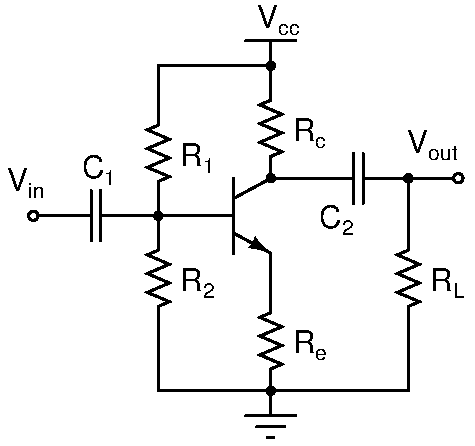
\includegraphics[height=0.50\textheight]{./schematics/npn_ac_common_emitter_amplifier}
		\end{figure}
	\end{column}
	\begin{column}<2->{.55\textwidth}
		Design rules
		\begin{itemize}
			\item chose gain $G=R_c/R_e$
			\item maximum output swing 
				\begin{itemize}
					\item $V_c=V_{cc} /2 $
				\end{itemize}
			\item quiescent current
				$I_c=(V_{cc}-V_c)/R_c= V_{cc}/2R_c$
			\item $R_c=V_{cc}/(2 I_c)$
			\item $R_e=R_c/G$ 
			\item we want $I_{R_1+R_2} \gg I_b$
				\begin{itemize}
					\item factor of 10 for a safe margin
						$I_{R_1+R_2} \ge 10 I_b = 10 I_c / \beta$
					\item
						$R_1+R_2 \le V_{cc} \beta /(10 I_c)$
				\end{itemize}
			\item $V_b=V_e \alert{+0.6 V}$
			\item 	$R_2 /(R1+R2) = V_b/V_{cc}$
		\end{itemize}
	\end{column}
\end{columns}
	
	}

\frame
{ \frametitle{AC-coupled common emitter (inverting) amplifier }
\begin{columns}[c]
	\begin{column}{.43\textwidth}
		\begin{figure}
			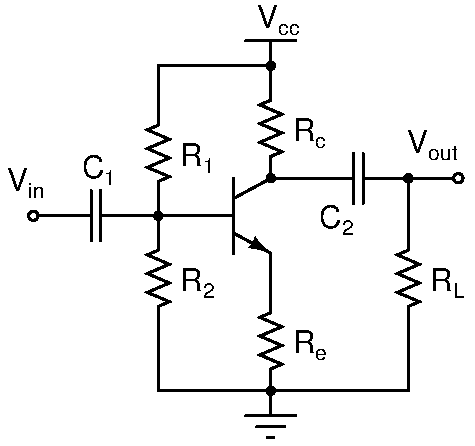
\includegraphics[height=0.50\textheight]{./schematics/npn_ac_common_emitter_amplifier}
		\end{figure}
	\end{column}
	\begin{column}<2->{.57\textwidth}
		\pause
		Input equivalent
		\begin{figure}
			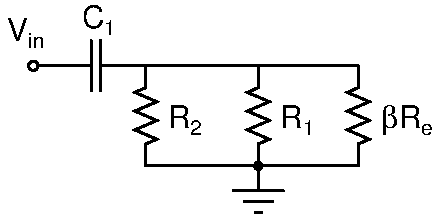
\includegraphics[height=0.20\textheight]{./schematics/ac_coupled_input}
		\end{figure}

		\pause
		Output equivalent
		\begin{figure}
			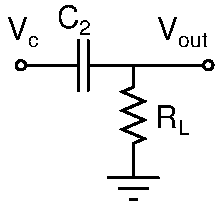
\includegraphics[height=0.20\textheight]{./schematics/ac_coupled_output_inv_amplifier}
		\end{figure}

		\pause
		See notes about AC-coupled emitter follower

	\end{column}
\end{columns}
	
	}

\begin{frame}
\frametitle{AC-coupled (inverting) amplifier with HF gain boost}
\begin{columns}[t]
	\begin{column}{.45\textwidth}
		From
		\begin{figure}
			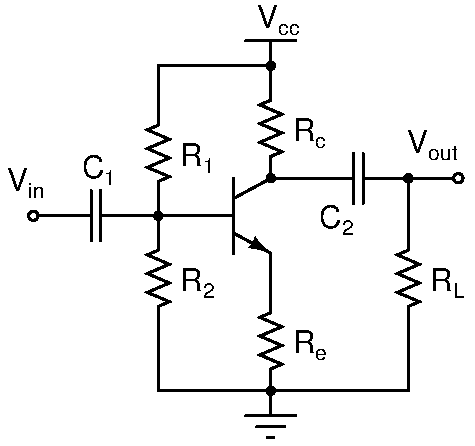
\includegraphics[height=0.50\textheight]{./schematics/npn_ac_common_emitter_amplifier}
		\end{figure}
	\end{column}
	\begin{column}{.45\textwidth}
		To
		\begin{figure}
			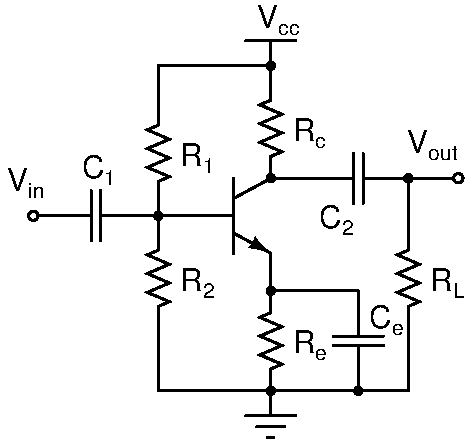
\includegraphics[height=0.50\textheight]{./schematics/npn_ac_common_emitter_amplifier_with_ac_boost}
		\end{figure}
		Think what happens with equivalent impedance of $R_e$ at high
		frequencies
	\end{column}
\end{columns}
\end{frame}

\end{document}
